
\chapter{Introduction}\label{CAPINTRO}

Persistent human papillomavirus (HPV) infections with genotypes 16 and 18 are responsible for about 70\% of all cervical cancer, with 40-85\% of other anogenital cancers: anal, penile, vaginal, and vulvar cancer, and also 16-28\% of the head and neck cancers.

HPV is a cause of other non malignant diseases, to mention genotypes 6 and 11 cause about 90\% of anogenital warts, and secondarily juvenile onset of recurrent respiratory papillomatosis.

There are three available vaccines: a quadrivalent (including HPV genotypes 16, 18, 6 and 11) and a bivalent vaccine (including genotypes 16 and 18) and a nonavalent (including genotypes 6, 11, 16, 18, 31, 33, 45, 52 and 58). All vaccines are efficacious to protect against precancerous lesions in the cervix, vulva or vagina; in addition, the quadrivalent and nonavalent prevent precancerous anal lesions, anal cancer and anogenital warts. These two lasts are indicated to vaccinate males from age 9 years.

In Spain HPV vaccine is given to adolescent girls as part of the national immunization programme, and is recommended at different age groups in different Autonomous Communities. Numerous cost-effectiveness studies of HPV-vaccination have been published in other countries. However, few studies include the prophylactic effect of all HPV-associated diseases, or the impact of vaccinating men.

There are countries that recommend also vaccinating boys in order to decrease the burden of disease in them. Some models have shown that the female vaccination program has some herd immunity and the impact of implementing the vaccination in males may not be cost effective, however not vaccinating males leaves them at risk of cancers, especially the groups that do not benefit of the herd immunity, as the males that have sex with males.
Besides, there is no economic analysis of the 9v program in Spain, and it is important from the decision making perspective.

Even with the high prevalence of sexually transmitted diseases there are few studies devoted to ascertain the structure of sexual networks and its role in disease transmission. Most studies are restricted to small communities such as the Jefferson High Schools project (P. S. Bearman et al., Chains of Affection: The Structure of Adolescent Romantic and Sexual Networks, American Journal of Sociology, 110(1) (2004) 44-91) or that of Likoma Island (S. Helleringer and H. P. Kohler, Sexual network structure and the spread of HIV in Africa: evidence from Likoma Island, Malawi, AIDS 21 (2007) 2323-2332).

Random network mathematical models may simulate the interactions and propagations of all these viruses through sexual contacts among a population of more than one million people (including heterosexual and homosexual populations). As this model is based upon a network instead of traditional continuous model approaches (E. H. Elbasha et al., Model for assessing human papillomavirus vaccination strategies,  Emerging. Inf. Dis.  2007; 13:28-41) we will be able to determine with higher accuracy the effect of vaccination in a short and large periods of time.

The purpose of this study was to assess the economic consequences of a national immunization program with publicly financed quadrivalent and nonavalent HPV vaccine for both boys and girls aged 12 years or a for only girls aged 12 years in Spain by means of a random network model. 

\section{Objectives}
Main objective:
\begin{itemize}
	\item To estimate the costs-effectiveness of vaccinating boys and girls at 11-12 years of age in Spain compared to vaccinate only girls.
\end{itemize}
Secondary objectives:
\begin{itemize}
	\item To estimate the impact of female vaccination on the epidemiology of HPV infections in males.
	\item To assess the impact of female vaccination on the epidemiology of males' anal head and neck and penis cancer.
\end{itemize}

\section{Methodology}

\subsection{Structure of the sexual network}

There are no published procedures to build a realistic sexual network from statistical data and to extend it to populations of medium to large size (up to one million individuals or more). This is a serious drawback to the development of simulations of sexually transmitted diseases. 

We have been working for the last years on an algorithm that takes into account the distribution of the number of partners and the age distribution among the partners. The statistical structure of these networks were obtained in terms of three parameters:

\begin{itemize}
	\item The number of individuals: N.
	\item The average number of lifetime sexual partners for men: k.
	\item A parameter we call $\alpha$ which it is related to the randomness in the assigment of partners.
\end{itemize}

The network is very sensitive to the parameter k but not to $\alpha$. For this reason it is very convenient for the simulations to use up-to-date surveys on sexual behaviour containing information about the distribution of partners in the population and the average number of partners of men and women. Based on the Spanish survey on health and sexual behaviour published in 2003, we inferred the value k=4.5 for Spain, smaller than the value k=5.5 obtained in American surveys. Results for different parameters for networks with N=5000 up to N=1,000,000 individuals can be found at the webpage:
\begin{center}
	\underline{\url{http://lsp.imm.upv.es}}
\end{center}

A typical result for N=5000 is displayed in Figure \ref{red1}.
\newline
The model considers three age groups:
\begin{itemize}
	\item 18-25 years
	\item 26-45 years
	\item 46-65 years
\end{itemize}

For each age group we also define a parameter T as a factor modulating the probability of transmission of VPH serotypes in a given sexual intercourse.
Standard demographic models developed by our research group for epidemic spreading simulations from local statistical data were also applied.

An important point is the construction of the men-to-men lifetime-sexual-partner network. This is relevant because of the high incidence of the disease in this group (anal cancer), the different sexual behaviour and promiscuity assumed and the possibility of transmitting the infection through bisexual contacts. 
As a source of statistical data on the behaviour of the homosexual population we will use the Durex's study and the European on-line survey for men having sexual relations with men (EMIS) for the particular case of Spain.
To incorporate this subpopulation in the network we will build the subnetwork using the same techniques developed for the heterosexual network.

\begin{figure}[ht]
	\centering
	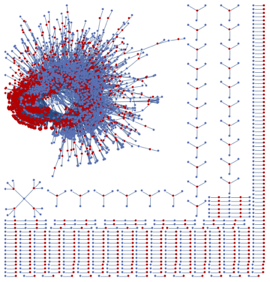
\includegraphics[scale=0.7]{IMG/red1.png}
	\caption{A heterosexual network for 5000 individuals. Men are represented by the red circles and women by the blue ones. Isolated couples and small clusters of relations are also displayed.}
	\label{red1}
\end{figure}  

\subsection{Evolution of the disease}
To analyze the spread of the infection of different HPV genotypes and the diseases associated with VPH infection in short and long term, we will take into account different scenarios according to the evolution of the population and sexual behavior. Progression and regressions from HPV infection to cervical dysplasia and precancerous lesions in states CIN1, CIN2 and CIN3 as well as localized, regional and distant cervical cancers will be incorporated into the model.  The burden of genital warts will also be considered.

The infection prevalence will be compared and fitted with real data obtained from recent studies (X. Castellsagu\'e et al., Prevalence and genotype distribution of human papillomavirus infection of the cervix in Spain: The CLEOPATRE study, J. Med. Virol. 2012 Jun; 84(6): 947-56). 

Costs associated with the diseases, both from the payers' perspective (Spanish Health System) and from the societal perspective will be incorporated into the model. Progression to cervical dysplasia or genital warts will also be considered in order to calculate the public health costs.
 
Costs will be obtained, when possible, from Spanish data. We will mainly use the Ley de Tasas de la Generalitat Valenciana, 2014 for common direct costs. Other costs may be obtained from local studies or publications.

\subsection{Impact of different Vaccination programs}

The final step will be to consider the modelling of vaccination strategies and their effect on the incidence and prevalence of the infection and diseases in both females and males. In a first step we will model vaccination with Gardasil for genotypes 6/11 and then for genotypes 16 and 18. Effectiveness of the vaccine to prevent infection and diseases will be extracted from the most up-to-dated bibliography. Initially only girls vaccinated at the age of 11-12 will be considered. A sensitivity analysis will include:
\begin{itemize}
	\item Different vaccine coverages ranging from 50% to 95%.
	\item pv: the percentage of initial protection.
	\item pp: the percentage of protection lost every month.
	\item tp: the time in which protection is totally lost (in months).
	\item Different vaccine prices.
	\item 3-5\% annual discount rate.
\end{itemize}

We will assume that protection (represented by f(x)) is lost linearly with time in terms of the function: 
\begin{align*}
f(x)=-\dfrac{pp}{tp}x+pv
\end{align*}
As part of the simulation we will update the protection for every individual in the network every time-step. Our time unit will be chosen as one month and individuals are to be classified in four states according to the VPH infection for each serotype:
\begin{itemize}
	\item Susceptible
	\item Infected
	\item Recovered
	\item Vaccinated
\end{itemize}

Later on, the progress to genital warts, precancerous lesions and cancer will also be taken into account as well as the influence of the manifested disease in the sexual behavior of these individuals. 

\section{Project roadmap and resources}

Simulations will be carried out in a computation cluster located at the Institute for Multidisciplinary Mathematics (IMM) based upon two new Intel Sandy Bridge platforms with 64 cores and 512 GB RAM each one. Further computational resources could be allocated in case they are needed for the larger networks by using distributed computational techniques (L. Acedo, Epidemic Random Network simulations in a distributed computing environment, A \& AA, 2013, ID 462801).

Deliverables will be scheduled as follows:

\begin{itemize}
	\item Implementation of an algorithm for generating realistic sexual networks including both heterosexuals and homosexual populations and validation of the algorithm using realistic statistical data surveys (end May 2016). 
	\item Simulation of the VPH infection for a large array of parameters and conditions, data analysis, fitting and sensitivity analysis in the absence of vaccination (June 2016).
	\item Fitting of the network (including vaccinated individuals) and predictions for several scenarios of coverage, population targets and age of vaccination, evolution of the VPH disease including CIN states, genital warts, cervical cancer and public health burden (July 2016).
	\item Cost-effectiveness analysis and final report (September 2016).
\end{itemize}

 
